\documentclass[12]{article}

\usepackage{graphicx}

\begin{document}

\title{Deep Q-Learning on Unity's Banana Environment}
\author{Christopher J. Miles}
\maketitle

\begin{abstract}
This report is done in fulfillment of the {\it Udacity Deep Reinforcement Nanodegree}. This project implements a Deep Q-Network (DQN) model and its variants such as DDQN, Dueling DQN on the Unity {\it Banana} environment. There are two observational state space encodings: ray-based perception and raw pixel information.
\end{abstract}




\section{Introduction}

Deep reinforcement learning (in particular, the DQN algorithm) is applied to the Unity Banana environment \cite{unity}.  The environment is a virtual 3D space where an agent is confined to a square region. The space is filled with randomly placed blue and yellow bananas. The objective is for the agent to collect as many yellow bananas as possible in the allotted time of 300 time steps. The agent receives a $+1$ reward for every yellow banana collected and a $-1$ for every blue banana collected. 

To solve this problem, variants of the Deep Q-Learning algorithm are employed \cite{Wang2016,Schaul2016,Mnih2015}. The details of each algorithms are discussed in the next section.

\section{Algorithms}

A `vanilla' DQN \cite{Mnih2015} is implemented as follows:

\section{Results}

\begin{figure}
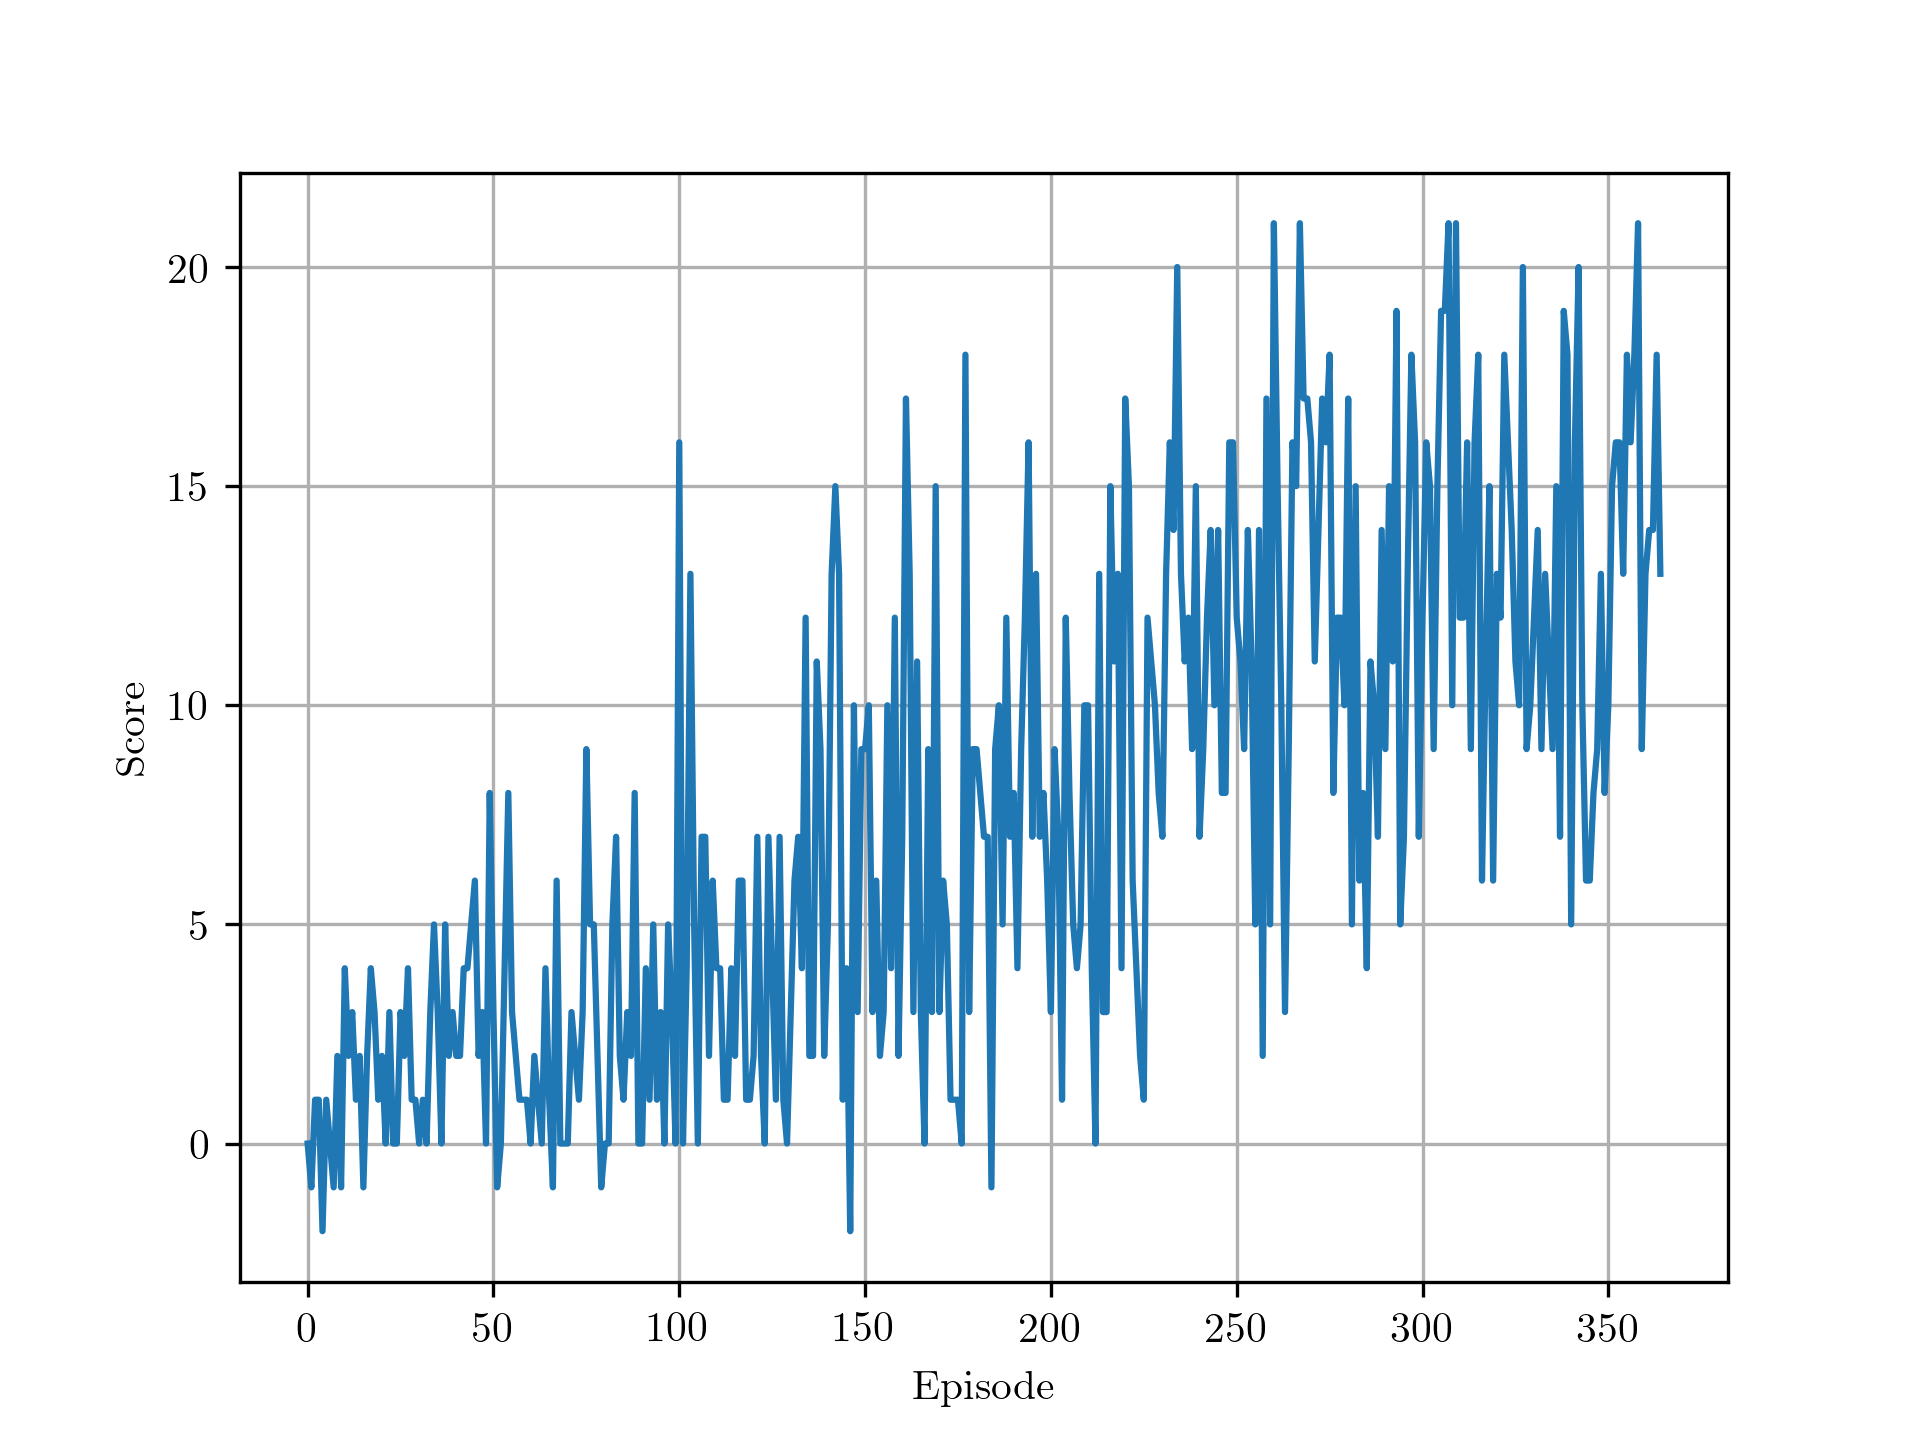
\includegraphics[width=0.9\textwidth]{images/scores_dqn}
\caption{Scores over episodes during DQN training.}
\end{figure}
\bibliographystyle{plain}
\bibliography{../../library}


\end{document}